% !TEX TS-program = xelatex
% !TEX encoding = UTF-8 Unicode
% !Mode:: "TeX:UTF-8"

%This file contains the LaTeX code of my laboratory report for my ICS II course.
%Author: 张作柏/Zuobai Zhang <17300240035@fudan.edu.cn>

% This is a simple template for a LaTeX document using the "article" class.
% See "book", "report", "letter" for other types of document.

\documentclass[12pt]{article} % use larger type; default would be 10pt

\usepackage[utf8]{inputenc} % set input encoding (not needed with XeLaTeX)

%%% Examples of Article customizations
% These packages are optional, depending whether you want the features they provide.
% See the LaTeX Companion or other references for full information.

%%% PAGE DIMENSIONS
\usepackage[top=1.05in, bottom=0.95in, left=0.90in, right=1.10in]{geometry}
%\usepackage{geometry} % to change the page dimensions
\geometry{a4paper} % or letterpaper (US) or a5paper or....
% \geometry{margin=2in} % for example, change the margins to 2 inches all round
% \geometry{landscape} % set up the page for landscape
%   read geometry.pdf for detailed page layout information

\usepackage{graphicx} % support the \includegraphics command and options

% \usepackage[parfill]{parskip} % Activate to begin paragraphs with an empty line rather than an indent

%%% PACKAGES
\usepackage{booktabs} % for much better looking tables
\usepackage{array} % for better arrays (eg matrices) in maths
\usepackage{paralist} % very flexible & customisable lists (eg. enumerate/itemize, etc.)
\usepackage{verbatim} % adds environment for commenting out blocks of text & for better verbatim
\usepackage{subfig} % make it possible to include more than one captioned figure/table in a single float
% These packages are all incorporated in the memoir class to one degree or another...

%%% HEADERS & FOOTERS
\usepackage{fancyhdr} % This should be set AFTER setting up the page geometry
\pagestyle{fancy} % options: empty , plain , fancy
%\renewcommand{\headrulewidth}{0pt} % customise the layout...
\lhead{}\chead{}\rhead{}
\lfoot{}\cfoot{\thepage}\rfoot{}

%%% SECTION TITLE APPEARANCE
\usepackage{sectsty}
\allsectionsfont{\sffamily\mdseries\upshape} % (See the fntguide.pdf for font help)
% (This matches ConTeXt defaults)

%%% ToC (table of contents) APPEARANCE
\usepackage[nottoc,notlof,notlot]{tocbibind} % Put the bibliography in the ToC
\usepackage[titles,subfigure]{tocloft} % Alter the style of the Table of Contents
\renewcommand{\cftsecfont}{\rmfamily\mdseries\upshape}
\renewcommand{\cftsecpagefont}{\rmfamily\mdseries\upshape} % No bold!
\usepackage{titletoc}
\titlecontents{section}
              [1.5cm]
              {\bf \large}%
              {\contentslabel{1.8em}}%
              {}%
              {\titlerule*[0.5pc]{$\cdot$}\contentspage\hspace*{0.6cm}}%
		   [\vspace{0.5em}]
\titlecontents{subsection}
              [1.8cm]
              {\normalsize}%
              {\contentslabel{2.0em}}%
              {}%
              {\titlerule*[0.5pc]{$\cdot$}\contentspage\hspace*{0.6cm}}%
		   [\vspace{0.4em}]
\titlecontents{subsubsection}
              [2.1cm]
              {\small}%
              {\contentslabel{2.5em}}%
              {}%
              {\titlerule*[0.5pc]{$\cdot$}\contentspage\hspace*{0.6cm}}%
		   [\vspace{0.4em}]


\usepackage[UTF8]{ctex}
\usepackage{fancyhdr}
\usepackage{enumerate}
\usepackage{indentfirst}
\usepackage{extramarks}
\usepackage{titling}
\usepackage{xcolor}
\usepackage{fontspec}
\usepackage[CJKbookmarks=true,colorlinks,linkcolor=black]{hyperref}
\setmainfont{Times New Roman}

%%% END Article customizations

%%% The "real" document content comes below...

%\title{\textbf{Digital Logic and Computer Design Report}}
\title{\textbf{Socket编程项目报告}}
\author{王鑫涛 17307130015\\张作柏 17300240035}
%\date{} % Activate to display a given date or no date (if empty),
         % otherwise the current date is printed 

\usepackage{amsmath}
\newcommand\calD{\mathcal{D}}
\newcommand\XX{\boldsymbol{\mathit{X}}}
\newcommand\qq{\boldsymbol{\mathit{q}}}
\newcommand\pp{\boldsymbol{\mathit{p}}}
\newcommand\yy{\boldsymbol{\mathit{y}}}
\newcommand\zz{\boldsymbol{\mathit{z}}}


\begin{document}
\begin{sloppypar}
\maketitle

\pagestyle{fancy}
\lhead{\textbf{{\thetitle}}}
\rhead{\textbf{\nouppercase{\firstleftmark}}}
\cfoot{\thepage}

\thispagestyle{empty}
\tableofcontents
\clearpage

\setcounter{page}{1}


\section{项目简介}

\subsection{项目要求}

{\bf 要求:}设计一个具体的协议(建议是应用层协议),采用标准SocketAPI编程来实现协议的功能。基于此协议,实现一个简单的聊天系统。

\begin{itemize}
	\item 协议的设计可以参考http等,语法语义相似。\vspace*{-1.5mm}
	\item 头部域自己设计,需要有完备的功能,服务器端要能理解客户端的各种请求,并有一定的错误处理机制。\vspace*{-1.5mm}
	\item 如无特殊情况,要求使用Python编程。\vspace*{-1.5mm}
	\item 如无特殊情况,不能使用额外封装的库。\vspace*{-1.5mm}
	\item 建议最好有图形界面。\vspace*{-1.5mm}
\end{itemize}

\subsection{技术栈与文件结构}

本次PJ按照要求使用Python3语言进行编程,通过socket包提供的借口实现协议的功能,前端设计使用PyQt5,具体介绍可参见第\ref{sec:detials}节。

项目目录下包含文件及其功能如下:
\begin{itemize}
	\item {\bf server.py:} 服务器端代码,通过调用socket包实现服务器的基本功能。\vspace*{-1.5mm}
	\item {\bf user.db:} 服务器端用于存储用户信息的数据库。\vspace*{-1.5mm}
	\item {\bf client.py:} 客户端代码,包括客户端协议的实现,与登录窗口、聊天窗口的调用。\vspace*{-1.5mm}
	\item {\bf Constant.py:} 定义了协议中用到的常数和相关的文件路径。\vspace*{-1.5mm}
	\item {\bf util.py:} 封装了信息、文件传递等socket基本功能,以便其他文件使用。\vspace*{-1.5mm}
	\item {\bf login\_win.py:} 登录窗口的布局与设计代码。\vspace*{-1.5mm}
	\item {\bf register\_win.py:} 注册窗口的布局与设计代码。\vspace*{-1.5mm}
	\item {\bf group\_win.py:} 创建新群聊界面的布局与设计代码。\vspace*{-1.5mm}
	\item {\bf chat\_ui.py:} 聊天界面的布局代码。\vspace*{-1.5mm}
	\item {\bf chat\_win.py:} 聊天界面的逻辑设计。\vspace*{-1.5mm}
	\item {\bf others.py:} 前端设计使用的封装组件类。\vspace*{-1.5mm}
\end{itemize}

服务器端、客户端的文件和头像分别存储在server、client文件夹中,image文件夹则存储启动聊天窗口需要用到的基本图片文件。

\subsection{功能介绍}

本次PJ我们使用socket编程,实现了一个基本的聊天系统,包括以下功能:
\begin{enumerate}
	\item {\bf 用户注册、登录功能}
	\item {\bf 广播信息:} 用户可在聊天大厅发送消息,所有在线用户都会收到该消息呢。 
	\item {\bf 登录登出提醒:} 用户的登录、登出信息会在聊天大厅进行通知。
	\item {\bf 私聊功能:} 通过点击在线用户列表中的头像、用户名,可切换到私聊模式,在此模式下可发送私聊信息,仅有该用户可收到。
	\begin{figure}[htbp]
		\centering
		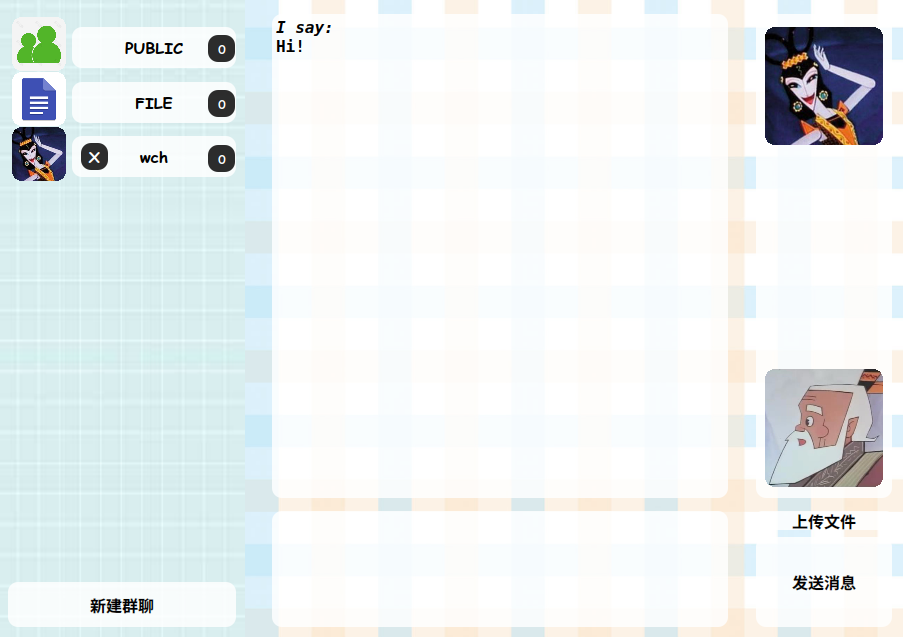
\includegraphics[width=0.7\linewidth]{figure/private.png}
		\caption{私聊界面}
	\end{figure}
	\item {\bf 群聊功能:} 通过‘新建群聊’按钮输入聊天室编号,可加入相应群聊聊天室(若当前该群聊未创建,则服务器端新建一个群聊聊天室)。群聊界面会显示当前群聊用户,在群聊中发送的信息,只会被该群聊中的用户接受。
	\begin{figure}[htbp]
		\centering
		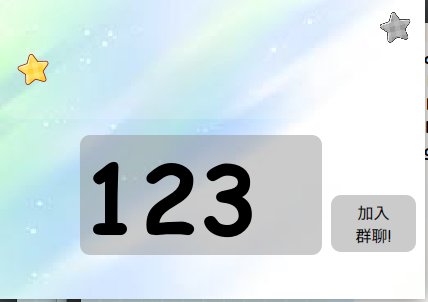
\includegraphics[width=0.4\linewidth]{figure/group.png}
		\caption{新建群聊界面}
	\end{figure}
	\item {\bf 传输、下载文件功能:} 用户可在大厅、私聊、群聊界面上传文件,界面中的相应用户会被提示新文件消息,并可在FILE界面中查看文件信息、选择是否进行下载。
	\begin{figure}[htbp]
		\centering
		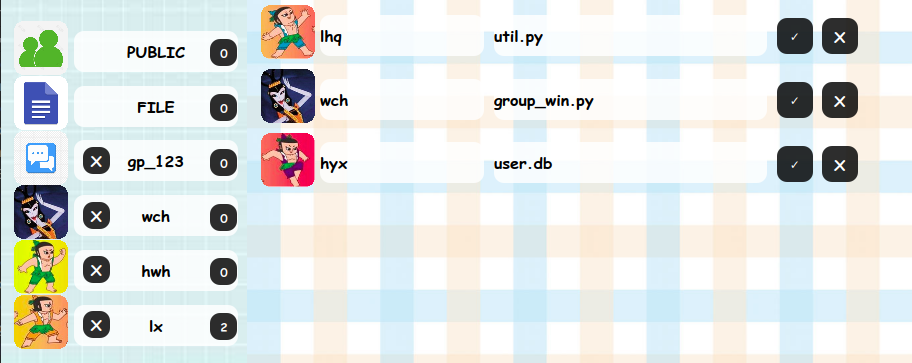
\includegraphics[width=0.8\linewidth]{figure/file.png}
		\caption{文件界面}
	\end{figure}
	\item {\bf 头像上传功能:} 用户可通过上传头像按钮,上传自己喜欢的头像,其他用户刷新页面即可查看最新头像。
	\item {\bf 聊天界面个性化设置:} 可通过配置本地文件来修改聊天室的背景、色调等,设置方法是将喜欢的图片放置image文件夹,然后修改Constant.py中的图片背景路径。
	\begin{figure}[htbp]
		\centering
		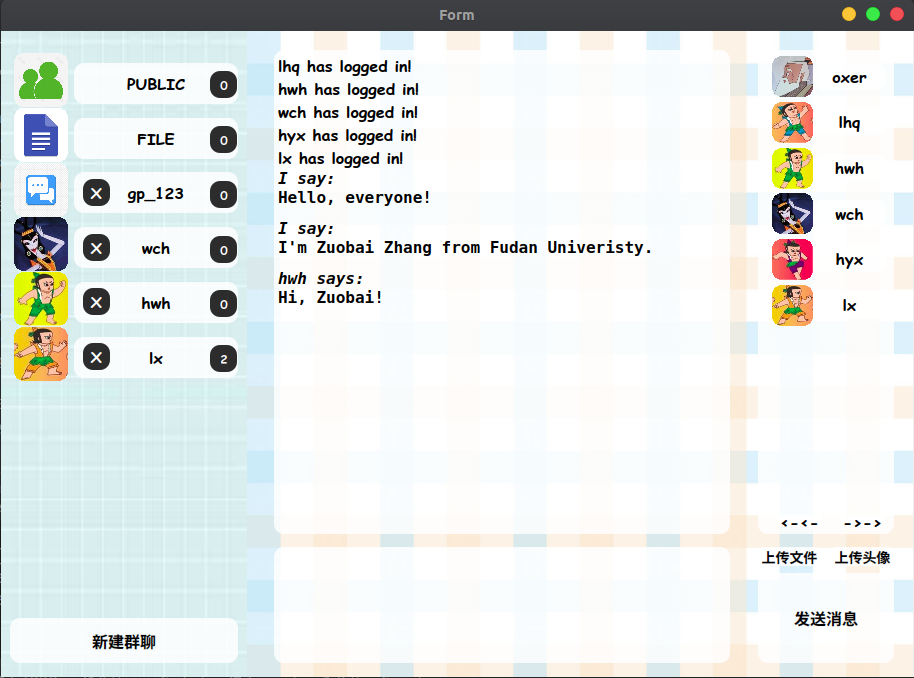
\includegraphics[width=0.9\linewidth]{figure/demo.png}
		\caption{聊天界面展示}
	\end{figure}
\end{enumerate}



\section{协议说明}

\subsection{客户端->服务器端}

客户端发往服务器的信息共16种,协议格式如下表所示。其中user表示当前动作涉及的用户,pwd表示密码,msg表示信息,groupid表示群聊编号,recv\_i表示第i个接受者用户名,fname、fsize、file分别表示文件名、大小、内容。

\begin{figure}[h]
	\centering
	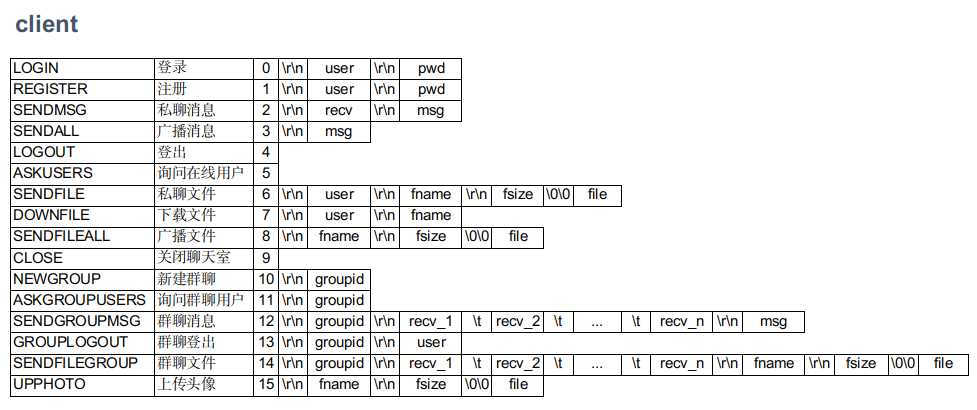
\includegraphics[width=0.95\linewidth]{figure/client.png}
	\caption{客户端协议}
\end{figure}
\vspace*{-1cm}

\subsection{服务器端->客户端}
服务器端收到客户端的请求后,回发送信息回复给客户端,其协议如下表所示。cnt表示用户个数,sender表示消息发送者,其余记号同上。
\begin{figure}[h]
	\centering
	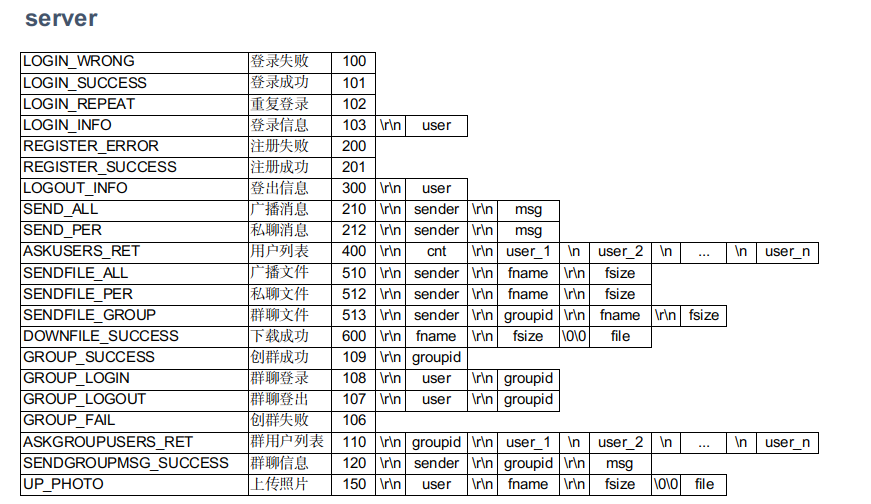
\includegraphics[width=0.9\linewidth]{figure/server.png}
	\caption{服务器端协议}
\end{figure}

\section{实现细节}
\label{sec:detials}

\subsection{后端}

\subsubsection{服务器端}

服务器端代码主要处理客户端发送来的信息,并给予相应的回复。服务器端首先需要创建用户数据库,以维护数据信息;而后连接对应端口并listen,每当发现一个新的连接,就将其记录在一个字典中;当用户登录后,修改字典,建立一个用户与连接之间的一一映射。之后,通过select函数收取端口发来的信息,并执行相应的操作。可能的信息与操作有:
\begin{enumerate}
	\item {\bf 登录操作:} 判断用户名是否存在于数据库中,用户名与密码是否匹配,若不存在或不匹配,则返回LOGIN\_WRONG信息;再判断用户是否已经登录,若已登录,则返回LOGIN\_REPEAT信息;若以上条件均满足,则将用户与相应连接绑定,并返回LOGIN\_SUCCESS信息。
	\item {\bf 注册操作:} 首先,判断用户名是否已存在与数据库中,若存在,则返回REGISTER\_ERROR。之后,将用户名与密码信息写入数据库,并返回REGISTER\_SUCCESS信息。
	\item {\bf 发送消息操作:} 包括发送私聊、广播、群聊消息。三者思路相仿,先找到receiver对应的连接,再向该链接发送信息。私聊、广播、群聊分别对应SEND\_PER、SEND\_ALL、SENDGROUPMSG\_SUCCESS消息。
	\item {\bf 上传文件操作:} 包括上次私聊、广播、群聊文件。同样,三者思路相仿,服务器先接受文件保存在服务器上,然后将文件的信息发送给相应的receiver。
	\item {\bf 下载文件操作:} 根据文件名确认要下载的文件,从服务器上读取文件内容,并转发给用户。
	\item {\bf 退出操作:} 包括退出群聊和退出聊天室。退出群聊时,将用户从相应群聊字典中移除,并向该群聊中用户发送GROUP\_LOGOUT信息以通知他们刷新页面。退出聊天室时,需要首先退出该用户所在的所有群聊,然后发送LOGOUT\_INFO信息在公屏通知登出信息。
	\item {\bf 询问用户操作:} 包括询问所有在线用户和询问群聊用户。服务器端使用列表和字典维护当前在线用户和每个群聊中的用户,直接通过ASKUSERS\_RET和ASKGROUPUSERS\_RET消息返回即可。
	\item {\bf 新建群聊操作:} 查询服务器端字典,若该群聊未存在,则新疆该群聊。若当前用户已加入该群聊,则返回GROUP\_FAIL信息,否则令该用户加入群聊,并返回GROUP\_SUCCESS信息,向群聊中的其他用户发送GROUP\_LOGIN信息。
	\item {\bf 上传头像操作:} 首先,接收头像并保存在服务器上。然后,发送头像文件给所有的用户,以更新用户头像。
\end{enumerate}

\subsubsection{客户端}

客户端需要兼顾聊天窗口显示和与服务器交互两项任务。首先,客户端连接服务器创建的端口,并打开登录窗口。用户可通过登录窗口上的注册按钮,打开注册窗口进行注册。用户登录后,关闭登录窗口,打开聊天窗口。可通过新建群聊按钮,打开新建群聊窗口。界面关闭时,会弹出对话框,选择是否确认退出。服务器端可能接受的信息和相应的操作有:
\begin{enumerate}
	\item {\bf 登录登出信息:} 若登录失败,则弹窗提醒对应错误。若登录成功,则退出登录窗口,打开聊天窗口。同时,发送ASKUSERS信号询问当前在线用户,以便更新用户列表。若收到LOGIN\_INFO或LOGOUT\_INFO,则可在聊天大厅发送用户的登录信息。
	\item {\bf 新消息信息:} 包括收到私聊、群聊、广播消息。在相应的窗口添加新消息,并更新未读信息条数。此外,若私聊窗口未创建,则会创建相应的私聊窗口。
	\item {\bf 新文件消息:} 包括收到私聊、群聊、广播文件。先在相应窗口添加文件收到的消息提醒,然后在FILE一栏中添加新文件,包括文件的发送者和文件名,供用户选择是否接收文件。接收时,则发送DOWNFILE信息。
	\item {\bf 文件下载信息:} 接收消息中传递的文件,并存放在客户端相应目录下。
	\item {\bf 创建群聊信息:} 当用户通过新建群聊窗口尝试连接新群聊时,发送NEWGROUP消息。客户端收到GROUP\_SUCCESS表示创建成功,打开群聊窗口,同时询问当前群聊中用户,否则为创建失败。同时,若收到GROUP\_LOGIN和GROUP\_LOGOUT信息,则在相应群聊中添加用户进入、退出群聊的通知。
	\item {\bf 用户信息:} 包括对所有在线用户列表和群聊用户列表的询问。根据返回的用户信息,刷新用户列表即可。
	\item {\bf 上传头像信息:} 接收头像文件,并刷新当前页面以更新用户的头像。
\end{enumerate}

\subsection{细节处理}

\subsubsection{编码方式}

由于传输的过程中是以比特的格式发送的,所以需要在发送前将协议字符串按utf-8格式编码为比特,在另一端进行相应的解码。但需要注意对协议信息不能直接解码,因为传输的信息中可能会包含文件,其内容未必是使用utf-8格式编码的,直接解码会出错。需要先找到协议头部与文件之间的分割符'$\backslash$ 0$\backslash$ 0',然后仅对头部进行解码。

\subsubsection{文件收发}

有的时候文件较大,不能在一个包中传送完毕,需要分多个包进行收发。同时,接受的缓冲区有大小限制,不能一次读完文件内容,需要进行多次的拼接。这里就需要通过文件大小这一属性来确认是否接收完毕。每次接收文件时,需先分离出文件的头部,包括文件名、文件长度等信息,然后不断接受文件,直到剩余字节数为0。


\subsubsection{粘包}

为提高网络效率,TCP在传包时默认会使用Nagle算法,对相邻的较小的包进行拼接,并且在接收方因为有缓冲区的存在,所以可能同时接受到多个相邻的包,这就出现了粘包的问题。如果相邻的包之间没有合适的间隔,则无法分开相邻包。正常的做法应是在协议头部加入包长度字段,以便于接收方分割粘连的包。但此处因为在设计的最后才遇到这一问题,重新修改协议有些费时,故此处可通过令服务器端在向同一个连接发送包时加入短暂的间隔时间,即可避免粘包的问题。

\subsection{前端}

初期的整体设计采用星空风格,以星空的照片、半透明白和半透明黑的框体搭配星星图像组件为主题。考虑到这种风格太过个性化而不够简约,这种风格只在登录框中得到了保留。而聊天框等其他窗体为了显得简约,使用了类似微信的简约风格。

前段和后端一样,使用Python语言进行编写。具体使用的工具包是PyQt,一个创建GUI应用程序的工具包,它是Python编程语言和Qt库的融合,有620多个类和6000个函数和方法。PyQt主要提供了图形组件、动画、以及使用户能够与图形界面交互的事件和信号量。

总体来说,PyQt的前端设计在许多方面上与原生的Web前端设计类似,通过创建组件、设置或修改组件的大小、名字、位置、字体甚至StyleSheet(大部分情况下和层叠样式表css一致)、控制组件的显示或隐藏实现了图形界面的大部分要求。交互方面,PyQt提供了事件及信号。使用最频繁的事件是鼠标点击,在PyQt中用item.clicked.connect(function)将鼠标点击事件绑定到一个函数,称为槽函数)上;信号则可以理解为事件的抽象,同样可以将信号通过connect(function)绑定到函数上。在槽函数中,我们可以调用sender = self.sender()来获取触发函数的组件,并可以通过sender来获取或修改组件的相关信息,也可以做其他指令,从而实现对前端的响应。

PyQt还提供了一款名为PyQtDesigner的软件以供实现可视化、所见即所得的前端开发:用户可以在软件中像搭积木一般进行GUI设计,然后通过相关指令生成相应的Python代码。然而在实践中过程中,我们发现该软件存在一些难以解释的问题,并且功能有限。但在早期,它生成的代码给我们展示了很好的代码组织结构。

基于这个组件的代码,我们进一步使用了前端布局(组件的创建和设置)与交互(事件与信号的处理、动画、组件的更新)解耦合的设计。在PyQt的框架中,最主要的类是窗体,而其他组件则是窗体对象的元素。我们一共设计了大小4种窗体:登录窗口,注册窗口,聊天窗口,以及创建会话窗口。每一个窗口在代码中是有继承关系的2个类。以聊天窗口为例,第一个类是Ui\_chatWindow,在构造函数中各组件并详细指明了各组件的位置、大小、名字、StyleSheet等信息;第二个类则叫ChatPage,继承了Ui\_chatWindow,并在此之上定义了信号、事件和信号的处理函数、动画函数、组件更新函数等。

PyQt里的动画可以通过类QPropertyAnimation创建,再使用setDuration(设置持续时间)、setStartValue/KeyValue/EndValue(起始位置大小、某一时刻位置大小、终点位置大小)来实现。除了平移,也可以使用旋转。我们设计了一个登陆动画,使登录框左上角的星星在按下登陆键时会沿着北斗七星的轨迹运动,并在到达北斗七星的位置时跳动。其实现就是通过让QPropertyAnimation对象依次运动到北斗七星的七个点(第一个点为StartValue,最后一个点为EndValue,其余点为KeyValue),并在到达KeyValue后进行放大和缩小运用,实现视觉上的跳跃感。

\begin{figure}[htbp]
	\centering
	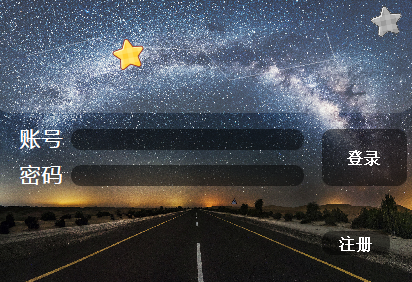
\includegraphics[width=0.6\linewidth]{figure/reg.png}
	\caption{登录界面展示}
\end{figure}

按照触发方式来说,除了由前端用户触发的函数,还有由后端服务器消息触发的函数。当后端消息需要对前端作出改动时,会通过我们定义的PyQt的信号来触发事件。信号对于外侧是透明的。比如,当socket发来消息说有新的用户向本地用户发送信息时,就会触发new\_conv信号,从而跳转到创建页面的函数。如果是一个已经存在的会话发来新的信息,则需要修改左侧聊天栏的未读消息数量。

按照功能来说,前端设计中的函数大体可以分为2类,处理数据、请求的函数和控制组件的函数,或者这2类的结合。处理数据的函数以简单的登陆为例,而控制组件的函数以聊天窗的换页为例。少数函数还会触发其他窗体的显示与隐藏,比如“注册”按钮的点击事件,或后端送来的登陆指令(将关闭登录窗口并显示聊天窗口)。

处理数据的函数逻辑非常简单,以登陆函数为例。在登陆的时候,我们从textEdit输入框组件中获取用户输入的信息(用户名和密码),然后通过socket发送相应的请求给后端。后续后端会对数据进行判断,如果数据符合数据库中的一个账号和密码,那就给本地socket发送登陆成功消息,否则发送登陆不成功消息。注册的逻辑也类似,只不过是向后端发送不一样的请求。更复杂的情况下,我们需要通过self.sender()获取触发事件或发送信号的组件再作出相应响应。比如说,左右两侧的用户id和头像的点击事件都被连接到了change\_page这个函数上,表示点击这些组件时会触发页面的转换。这个时候change\_page函数就需要通过self.sender()获取触发事件的组件,然后从我们对sender设置的名字中获取相关信息,包括类型、序号等,再根据不同的类型作出不同的响应。

\begin{figure}[htbp]
	\centering
	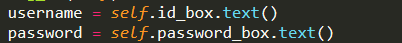
\includegraphics[width=0.6\linewidth]{figure/fig1.png}
\end{figure}

前端设计中的难点在于聊天窗,因为其他框体的组件是固定的,而聊天窗为了实现在不同页面的切换,组件是不固定的;同时,对于不同类型的聊天(公聊、私聊、群聊以及文件传输界面),组件的类型和数目也是不同的,还需要记载组件信息的数据结构,这就要求不同的处理。早期实现时,没有考虑到后面要加的群聊功能,因此代码结构相对简单,这给后期添加功能带来了一些问题,不得不重构代码。

实现切换界面功能的是flush\_page函数,它的参数为chat\_index,是聊天页面的编号。组件命名符合规则:前缀说明组件的类型,后缀说明组件的序号。当用户点击某个可以切换页面的组件时,或许是左侧聊天列表的项目,或许是右侧用户列表的项目,或许是用户名,或许是头像,我们都可以通过self.sender()获取用户点击的组件信息。如果对应的用户已经存在一个会话,那么该会话已有相应的页面编号,就使用flush\_page(页面编号)跳到这一页。否则,则为之创建一个新会话。flush\_page函数会将当前聊天页面的所有组件(会话列表是独立于所有页面的,因此不会被隐藏)隐藏,然后根据新页面的类型,展示其对应的组件。

关键的数据结构有conv\_list,conv\_people,conv\_pages,grp\_userbtn\_list,grp\_user\_list,grp\_page,conv\_type。其中,conv\_list[i]记录第i个会话对应的信息(数据),包括用户名、头像存储路径和消息数量等。conv\_pages[i]则是组件的列表,记录了第i个会话的所有组件。conv\_type[i]指明了第i个会话的类型是公聊、群聊、私聊或文件传输界面,以便作出相应处理。grp\_userbtn\_list、grp\_user\_list和grp\_usepage是字典,分别记载了对应位置的群聊会话的组件列表、群聊用户列表和群聊用户页数(即展示第几页的群聊用户)。当新的聊天界面被创建时,相应的数据结构会被创建,然后左侧列表中会出现切换聊天界面的组件。当一个聊天界面被删除时,相应的数据结构也会被删除,然后切换回公聊频道。

在早期使用了用户与组件绑定的策略,尤其是用户会与头像框、用户名的label组件一一对应,而后期为了解决当用户过多时的换页功能,意识到用户数量可能无上限,所以取消了这种绑定,使组件与用户解耦合,而在切换用户列表页的时候刷新头像框的图片和用户名label的文本,并在后台记录相关信息。

我们还可以重写PyQt本身定义的事件。比如,通过重写窗体的resize事件,使组件可以随窗体大小等比放缩;通过重写paint事件,可以在窗体上进行绘图;通过重写鼠标事件,可以实现窗体的自由拖动。

\section{总结}

本项目使用socket编程的方法实现了一个简易聊天室,界面简洁,功能便利,完成了项目的基本要求。本项目由王鑫涛和张作柏两人合作完成,其中王鑫涛负责前端的设计,张作柏负责后端的设计,前后端的交互则由两人共同完成。在本项目中,两人学习并掌握了socket编程、PyQt的使用等技能,收获颇丰。需要吸取教训的一点时,前期由于两人对项目没有系统地进行设计规划,所以导致文件的结构不清晰,代码比较混乱,无奈下只能重构,当然这也与Qt本身并不适合多人合作有关。




\end{sloppypar}
\end{document}
